\subsection{Introducci\'on} 

Cada participante de una competencia debe cruzar un puente dando saltos de tabl\'on en tabl\'on, con la limitaci�n de que pueden saltar como m\'aximo una cantidad fija de tablones por vez. Sin embargo algunos de estos tablones est\'an rotos. El objetivo del ejercicio es dar un algoritmo que nos devuelva un recorrido por los tablones del puente el cual sea m�nimo en la cantidad de saltos requeridos para poder cruzarlo con una complejidad temporal de \Ode{n} donde n es la cantidad de tablones del puente.

\subsection{Ejemplos y Soluciones}

Sea un puente de 14 tablones representado por el siguiente vector de 0 y 1, \verb+[0,0,0,1,1,0,0,1,0,1,0,0,1,0]+ llamado \verb+vector_puente+, donde 1 representa que el tabl\'on esta roto y 0 sano, y la primer posici�n del mismo el inicio del puente y la �ltima el fin del mismo. Adicionalmente sabemos que la cantidad m�xima de tablones que el participante puede saltar son 3 tablones.

Nuestro algoritmo va a encontrar la soluci�n de la siguiente forma:
En cada paso el algoritmo goloso busca quedarse con la solucion optima, esta es el salto maximo que el participante puede saltar, con lo cual en cada paso de nuestro algoritmo lo que realiza es intetar este salto si es factible, en caso que el tablon esta sano saltamos a ese tablon y continuamos de manera iterativa, caso contrario comenzamos a revisar desde el salto maximo acercandonos tablon por tablon hasta la posicion actual hasta encontrar un tablon sano. Esto podria no ocurrir y en ese caso quiere decir que hay una cantidad de tablones rotos mayor al salto maximod el participante y en esta situacion no tenemos solucion.

\subsection{Desarrollo}

Para la soluci\'on de este problema recurrimos a la tecnica de algoritmos voraces, donde en cada paso en la construccion a la solucion obtenemos el mejor salto. 
Por el enunciado sabemos que tenemos n tablones, el participante puede saltar C tablones de una sola vez y cuales son las posiciones de los tablones rotos.Nos armamos un arreglo donde cada posici\'on representa un tabl\'on, en el cual guardamos 0 y 1 para indicar su estado (sano o roto respectivamente) llenando el mismo seg\'un la entrada, llamemoslo puente.
Nuestro algoritmo ira recorriendo el puente tratando de hacer el mayor salto cuando este es posible, dependiendo si el tablon al que iria a parar el participante esta sano, en caso contrario comenzamos a iterar los tablones desde este salto maximo hacia donde se encuentra parado el participante uno por uno hasta encontrar un tablon sano.\\
Para cada al cual se salta se guarda su posicion en una lista siempre insertando atras de la misma, una vez que cruzo participante cruzo todo el puente se devuelve esta lista como la sucesion de saltos realizada por el participante, en caso de no ser factible ya que en una seccion del puente la cantidad de tablones rotos consecutivos es mayor a el salto maximo se devuelve no, ya que no tiene solucion.


\subsection{Complejidad}
El siguiente es un pseudo-c\'odigo de nuestro algoritmo.\\


 \begin{algorithm}
  \begin{algorithmic}[1]\parskip=1mm
 \caption{ \\Saltos( salto\_Maximo : natural, puente : arreglo(1's y 0's), distancias: arreglo(naturales) , cantidadTablones : natural)}
 		\STATE{Si saltoMax $>$ cantidadTablones ~~~O(1)}   
 		\STATE{\quad devolver 1}
 		\STATE{SI NO}
 		\STATE{SI existe una cantidad de tablones rotos mayor o igual a salto\_maximo en algun lugar del puente}
 		\STATE {\quad no existe solucion}
 		\STATE{nueva listaDeSaltos}
 		\STATE{\quad mientras posActual $<$ n $\&\&$ posActual >= 0 ~~~O(n)} 
 			\STATE{\quad\quad SI puente(posActual) == 0 }
 			\STATE{\quad\quad\quad Agrego posActual a Lista de Saltos}
 			\STATE{\quad\quad\quad le sumo a posActual el largo del salto }
 			\STATE{\quad\quad SI NO  }
 			\STATE{\quad\quad Le resto uno a PosActual}
 			\STATE{\quad\quad Devolver listaDeSaltos}
  \end{algorithmic}
  \end{algorithm}	
 Todas las asignaciones y comparaciones son en \Ode{1} como esta marcado en el pseudocodigo, ya que son n�meros naturales y est�n acotados por la cantidad de tablones\\
 En la linea 4 para revisar si la cantidad de tablones rotos es mayor o igual a el salto maximo en alguna parte del puente se realiza un ciclo que cuenta la cantidad de tablones rotos consecutivos, en caso de que se encuentre con uno sano resetea el contador y comienza de nuevo a contar, en el caso que el contador llegue a superar el salto maximo se devuelve que no tiene solucion. Esto se realiza con un solo ciclo y la complejidad es \Ode{n}. 
 El ciclo de las lineas 7 - 13 se realiza n veces en el peor caso con lo cual la complejidad total del algoritmo es \Ode{n}, ya que los dos posibles peores casos son, cuando el puente esta sano y salta de a un tablon por vez, o cuando los unicos tablones sanos son en las posiciones 1, Salto Maximo +1 , 2*(salto Maximo +1)..., de esta manera siempre salta el maximo y recorre los tablones hasta el primero para encontrar el sano dando como resultado que recorre todo el puente para encontrar los saltos.
 

 
\subsection{Demostraci\'on}
Para la prueba de correctitud, queremos demostrar que nuestro algoritmo siempre encuentra una suceci�n de saltos que es la menor posible.

Luego para demostrar por absurdo, supongamos que no es as�. Dicho mas formalmente, existe una suceci�n $V=\{v_1,v_2,...,v_i\}$ de saltos tal que es menor a la suceci�n $W= \{w_1,w_2,...,w_i, w_{i+1},...,w_j\}$ que encuentra nuestro algoritmo.

Por condiciones del problema sabemos el tablon al que queremos saltar no puede estar a distancia mayor a $k$ (el salto maximo posible), esto significa que:

$$v_1 \leq k$$
$$v_2 - v_1 \leq k$$
$$...$$
$$v_i - v_{i-1} \leq k$$

Sumando:

$$v_1 \leq k$$
$$v_2 \leq 2.k$$
$$...$$
$$v_i \leq i.k$$

Pero nuestro algoritmo, en cada paso, salta la mayor cantidad de tablones posibles y de all� comienza a retroceder hasta encontrar uno sano, dado que $v_1,v_2,...,v_i$ deben ser tablones sanos, los tablones elegidos por nuestro algoritmo estar�n acotados de esta manera:

$$ v_1 \leq w_1 \leq k $$ 
$$ v_2 \leq w_2 \leq 2.k$$
$$...$$
$$ v_i \leq w_{i} \leq i.k$$

Pero entonces, esto quiere decir que nuestro algoritmo encuenta una suceci�n de saltos, para los cuales siempre se salta por lo menos, la misma cantidad de tablones que en la suceci�n $V$. Luego nuestro algoritmo encuentra una soluci�n $W$ que tiene, como mucho, $k$ saltos.

Dado que supusimos que nuestro algoritmo encuntraba una suceci�n que era peor a $V$, abusrdo.

Luego nuestro algoritmo encuentra siempre una suceci�n de saltos que es minima.

\newpage			

\subsection{Experimentacion}
Para la experimentaci�n del problema en cuesti�n se realizaron los dos test de peores casos como se menciono en la seccion de complejidad, el primero teniendo en cuenta el  caso que todos los tablones del puente est�n sanos y el salto m�ximo del participante sea uno, para esto se fijo el salto m�ximo y se crearon 100 instancias de puentes sanos en tama�os que van del 1 al 100 luego se midieron los tiempos de ejecuci�n dando como resultado el siguiente gr�fico \\
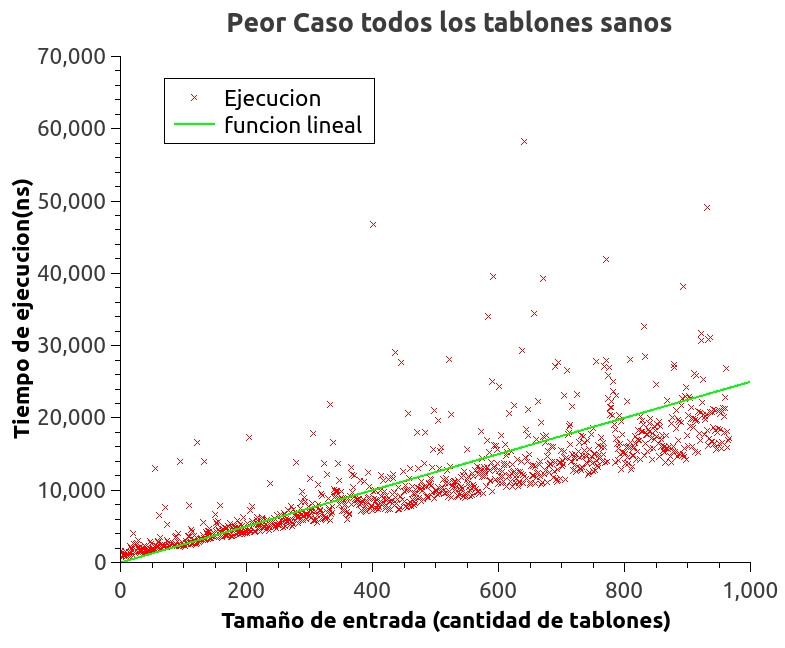
\includegraphics[scale=0.7]{Ej1/sanos.jpg}\\
Como puede verse en el gr�fico su complejidad esta en el orden lineal como puede compararse con la funci�n, en el gr�fico puede observar que algunos casos excede el orden, este ruido se debe a que puede haber ovaciones donde el sistema operativo este realizando otras tareas y afecte el orden de ejecuci�n.
En el segundo test, se realizo el segundo caso mencionado en la seccion complejidad y dando como resultado un grafico con complejidad del orden lineal como se puede observar en el siguiente grafico.
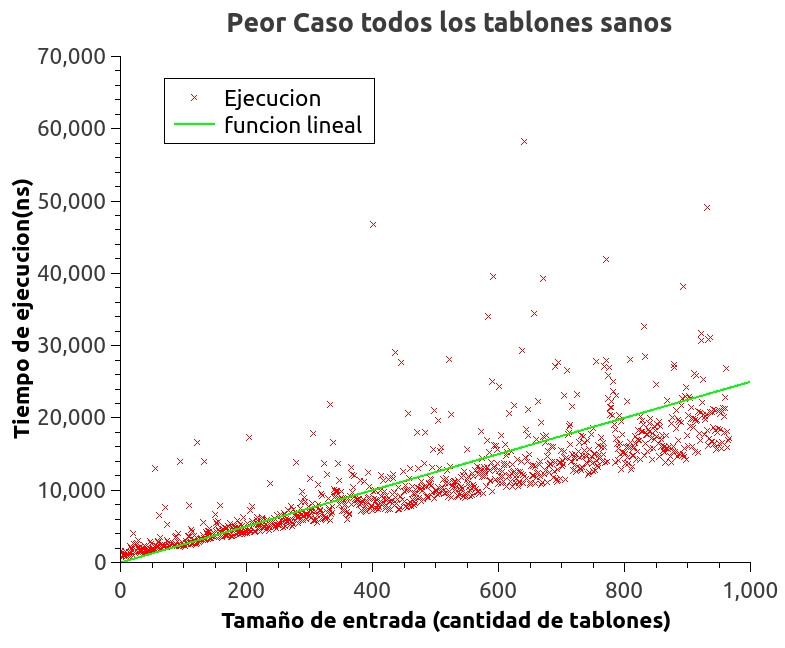
\includegraphics[scale=0.7]{Ej1/sanos.jpg}\\

Para el tercer test se realizo un test aleatorio, para poder observar el comportamiento de todos los casos posibles, para esto se crearon 1000 instancias, en las cuales el tama�o del puente fue creciendo de 1 a 1000  y el salto m�ximo es un numero random entre 1 y la cantidad de tablones del puente para poder obtener tambi�n casos que no sean soluci�n, dando comer resultado el siguiente gr�fico.
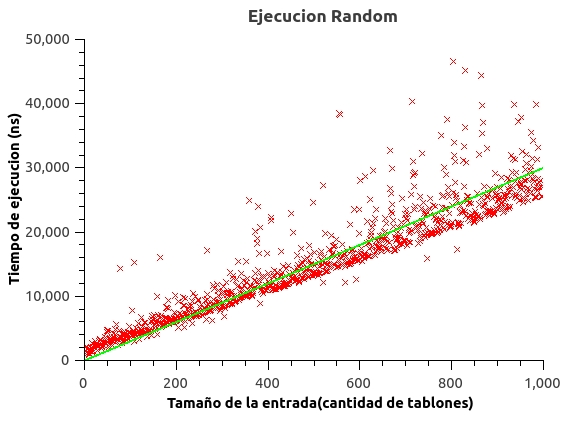
\includegraphics[scale=0.7]{Ej1/Random.jpg}\\

Puede observarse que al igual en el test anterior el orden de complejidad esta en el orden lineal, de esta manera podemos concluir que nuestro algoritmo cumple con los ordenes de complejidad impuestos por el enunciado.

